\documentclass[letterpaper,11pt]{article}
\oddsidemargin -1.0cm \textwidth 17.5cm

\usepackage[utf8]{inputenc}
\usepackage[activeacute,spanish, es-lcroman]{babel}
\decimalpoint
\usepackage{amsfonts,setspace}
\usepackage{amsmath}
\usepackage{amssymb, amsmath, amsthm}
\usepackage{comment}
\usepackage{float}
\usepackage{amssymb}
\usepackage{dsfont}
\usepackage{anysize}
\usepackage{multicol}
\usepackage{enumerate}
\usepackage{graphicx}
\usepackage[left=1.5cm,top=2cm,right=1.5cm, bottom=1.7cm]{geometry}
\setlength\headheight{1.5em} 
\usepackage{fancyhdr}
\usepackage{multicol}
\usepackage{hyperref}
\usepackage{wrapfig}
\usepackage{subcaption}
\usepackage{siunitx}
\usepackage{cancel}
\usepackage{mdwlist}
\usepackage{svg}
\pagestyle{fancy}
\fancyhf{}
\renewcommand{\labelenumi}{\normalsize\bfseries P\arabic{enumi}.}
\renewcommand{\labelenumii}{\normalsize\bfseries (\alph{enumii})}
\renewcommand{\labelenumiii}{\normalsize\bfseries \roman{enumiii})}


\begin{document}

\fancyhead[L]{\itshape{Facultad de Ciencias F\'isicas y Matem\'aticas}}
\fancyhead[R]{\itshape{Universidad de Chile}}

\begin{minipage}{11.5cm}
    \begin{flushleft}
        \hspace*{-0.6cm}\textbf{FI1000-1 Introducción a la Física Clásica}\\
        \hspace*{-0.6cm}\textbf{Profesora:} Paulina Lira\\
        \hspace*{-0.6cm}\textbf{Auxiliares:} Alejandro Cartes \& Juan Cristóbal Castro\\
        \hspace*{-0.6cm}\textbf{Ayudantes:} Francisca Bórquez \& Catalina Molina\\
    \end{flushleft}
\end{minipage}

\begin{picture}(2,3)
    \put(366, 10){\includegraphics[scale=0.9]{2020-1/Imágenes/logo/dfi-fcfm.pdf}}
\end{picture}

\begin{center}
	\LARGE\textbf{Auxiliar \#6}\\
	\Large{Cuerdas, Poleas y Ley de Hooke}
\end{center}

\vspace{-1cm}
\begin{enumerate}\setlength{\itemsep}{0.4cm}

\rfoot[]{pág. \thepage}

\item[]

\item Dos bloques unidos por una cuerda ideal, que pasa por una polea, descansan sobre planos lisos como se muestra en la Figura~\ref{fig:p1}. Si $M>m$ y $\alpha <\beta$, determine:
    \begin{enumerate}
        \item El sentido de movimiento del sistema
        
        \item La aceleración de los bloques
        
        \item Tensión de la cuerda
    \end{enumerate}

\item Considere el montaje mostrado en la Figura~\ref{fig:p2}. La masa $m_1$ es $n$ veces la masa $m_2$. Considerando poleas y cuerdas ideales, determine la aceleración de la masa $m_2$ a medida que $m_1$ desciende desde una altura $h$. ¿Cuál es la altura máxima del suelo a la que podrá subir $m_2$?

\begin{figure}[h!]
    \centering
    \begin{subfigure}[t]{0.4\textwidth}
        \centering
        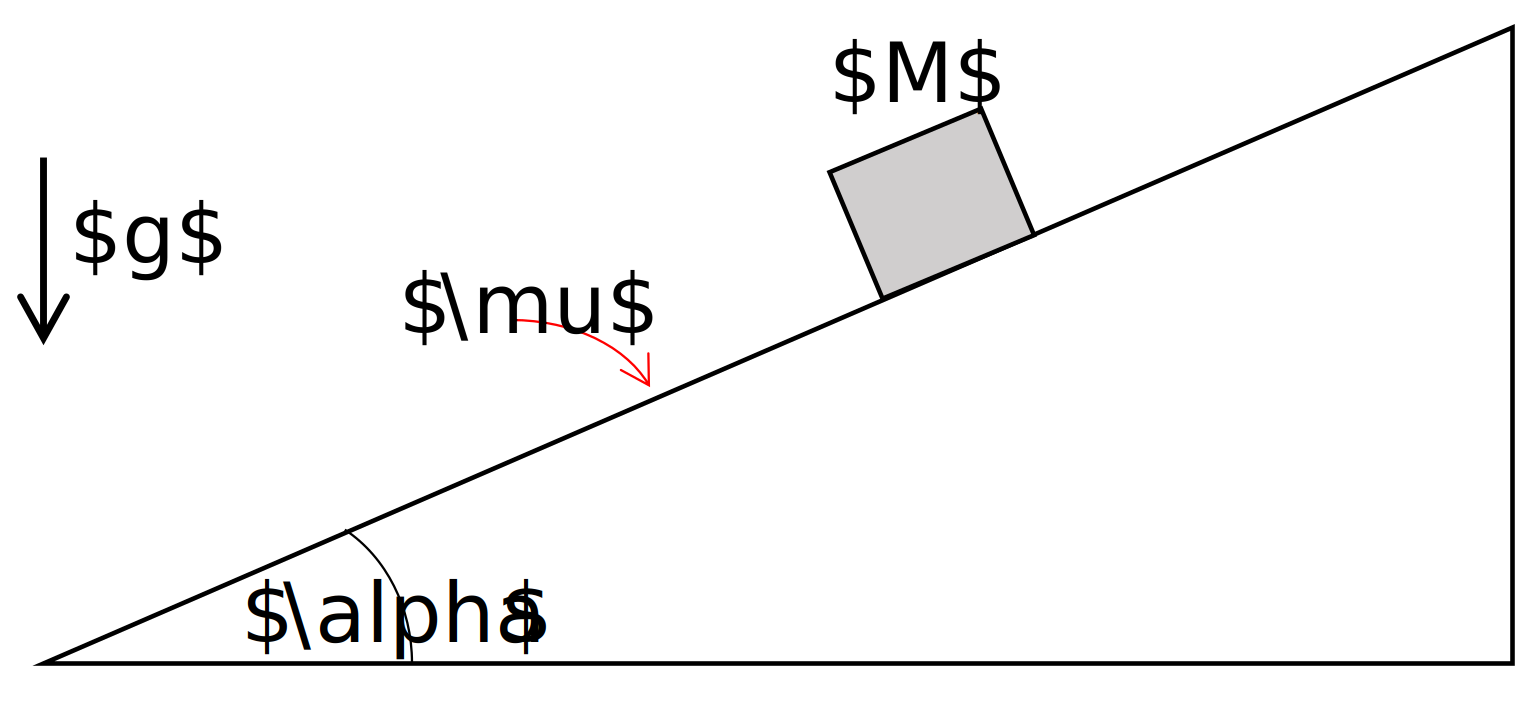
\includegraphics[width=0.9\linewidth]{2021-1/Imagenes/aux6/p1.pdf}
        \caption{P1}
        \label{fig:p1}
    \end{subfigure}
    \hspace{0.5em}
    \begin{subfigure}[t]{0.15\textwidth}
        \centering
        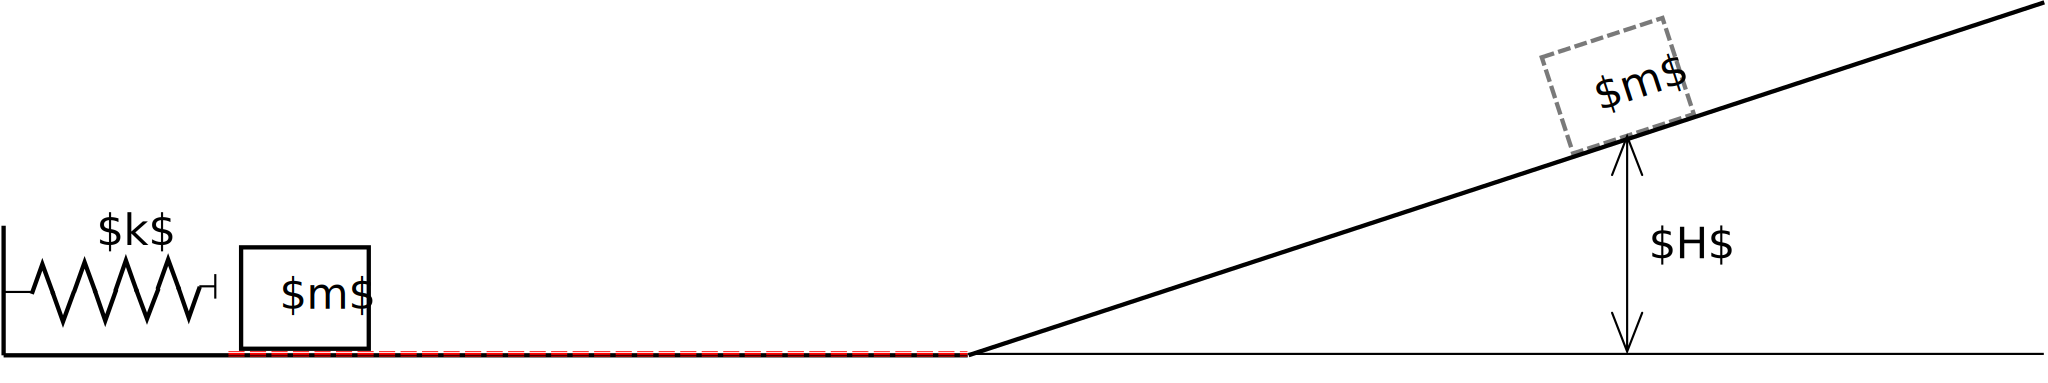
\includegraphics[width=0.75\linewidth]{2021-1/Imagenes/aux6/p2.pdf}
        \caption{P2}
        \label{fig:p2}
    \end{subfigure}
\end{figure}

% \item Dos esferas están unidas por una cuerda ideal que pasa por dos orificios de una mesa horizontal, con la geometría que se muestra en la figura \ref{fig:p3}. Una de las esferas, de masa $\lambda m$, cuelga verticalmente. Mientras que la otra esfera, de masa $m$, gira con velocidad angular constante $\omega$ a una distancia $L$ de la mesa. Determine el valor de $\omega$ y el ángulo $\beta$ si la esfera de masa $\lambda m$ está quieta, ¿qué condición debe cumplir $\lambda$ para que sea posible el sistema descrito?.

\item En presencia de la gravedad terrestre, una bolita de masa $m$ es sostenida mediante un resorte de constante elástica $k$ y longitud natural $L$, como se muestra en la figura \ref{fig:p3}. El conjunto se dispone dentro de un tubo de paredes lisas inclinado en un ángulo $\beta$ con respecto a la vertical. El tubo se hace girar con velocidad angular constante $\omega$ y la bolita mantiene una trayectoria circunferencial. El extremo superior $Q$ del resorte se ubica en el eje de rotación. Determine la elongación $\Delta$ del resorte y discuta la posibilidad de que $\Delta = 0$

\item De las dos siguientes configuraciones de la figura \ref{fig:p4}, ¿cuál de ellas produce la mayor elongación del extremo inferior?

\begin{figure}[H]
    \centering
    \begin{subfigure}[t]{0.45\textwidth}
        \centering
        \svgpath{../../2021-1/Imagenes/aux9/}
        \includesvg[width=0.7\linewidth]{resorte1.svg}
        \caption{P3}
        \label{fig:p3}
    \end{subfigure}
    \begin{subfigure}[t]{0.45\textwidth}
        \centering
        \includegraphics[scale=0.2]{2021-2/img/aux6/resortes.png}
        \caption{P4}
        \label{fig:p4}
    \end{subfigure}
\end{figure}

\item Cuatro partículas idénticas de masa $m$ se unen mediante resortes idénticos de masa nula, constante elástica $k$ y longitud natural $L$. El sistema toma la forma cuadrada de la figura mientras rota en torno a su centro con velocidad angular $\omega$. Calcule la elongación experimentada por los resortes.

\begin{figure}[H]
    \centering
    \svgpath{../../2021-1/Imagenes/aux9/}
    \begin{subfigure}[t]{0.45\textwidth}
        \centering
        \includesvg[width=0.4\linewidth]{resorte1.svg}
        \caption*{Figura P1}
    \end{subfigure}
    \hspace{0.1em}
    \begin{subfigure}[t]{0.45\textwidth}
        \centering
        \includesvg[width=0.5\linewidth]{cuadrao.svg}
        \caption*{Figura P2}
    \end{subfigure}
\end{figure}


\item~\textbf{[Propuesto]} Una esfera de masa $m$ es mantenida en la posición $A$ por dos cuerdas. Sea $T_A$ la tensión de la cuerda indicada en la figura \ref{fig:p4}. Se corta la cuerda horizontal y el péndulo oscila hasta la posición $B$. ¿Cuál es la razón de las tensiones $T_B/T_A$?

\begin{figure}[H]
    \centering
    \begin{subfigure}[t]{0.42\textwidth}
        \centering
        \svgpath{../../2021-2/img/aux4}
        \includesvg[width=1.0\linewidth]{mesa.svg}
        \caption{P3}
        \label{P3}
    \end{subfigure}
    \hspace{0.5em}
    \begin{subfigure}[t]{0.42\textwidth}
        \centering
        \svgpath{../../2021-2/img/aux4}
        \includesvg[width=0.8\linewidth]{pendulos.svg}
        \caption{P4}
        \label{P4}
    \end{subfigure}
\end{figure}



% Para imágenes vectoriales -> el texto tiene que estar en LaTeX
% \begin{figure}[htbp]
%   \centering
%   \svgpath{../Imagenes/ejercicios}  -> .. irse pa'trás 
%   \includesvg{ej5.svg}
% \end{figure}

\end{enumerate}
\end{document}
